\documentclass[a4paper,10pt]{article}
\usepackage{fullpage}
\usepackage[british]{babel}
\usepackage[T1]{fontenc}
\usepackage{amsmath}

\usepackage{mathtools}
\DeclarePairedDelimiter{\ceil}{\lceil}{\rceil}

\usepackage{amssymb}
\usepackage[T1]{fontenc}
\usepackage[utf8]{inputenc}
%\usepackage{amsthm} \newtheorem{theorem}{Theorem}
\usepackage{color}
\usepackage{float}
\usepackage{todonotes}
\usepackage{caption}
\DeclareCaptionFont{white}{\color{white}}
\DeclareCaptionFormat{listing}{\colorbox{gray}{\parbox{\textwidth}{#1#2#3}}}
\captionsetup[lstlisting]{format=listing,labelfont=white,textfont=white}
\usepackage{alltt}
\usepackage{listings}
 \usepackage{aeguill}
\usepackage{dsfont}
%\usepackage{algorithm}
\usepackage[noend]{algorithm2e}
%\usepackage{algorithmicx}
\usepackage{subfig}
\lstset{% parameters for all code listings
language=Python,
frame=single,
basicstyle=\small, % nothing smaller than \footnotesize, please
tabsize=2,
numbers=left,
% framexleftmargin=2em, % extend frame to include line numbers
%xrightmargin=2em, % extra space to fit 79 characters
breaklines=true,
breakatwhitespace=true,
prebreak={/},
captionpos=b,
columns=fullflexible,
escapeinside={\#*}{\^^M}
}


% Alter some LaTeX defaults for better treatment of figures:
    % See p.105 of "TeX Unbound" for suggested values.
    % See pp. 199-200 of Lamport's "LaTeX" book for details.
    % General parameters, for ALL pages:
    \renewcommand{\topfraction}{0.9}	% max fraction of floats at top
    \renewcommand{\bottomfraction}{0.8}	% max fraction of floats at bottom
    % Parameters for TEXT pages (not float pages):
    \setcounter{topnumber}{2}
    \setcounter{bottomnumber}{2}
    \setcounter{totalnumber}{4} % 2 may work better
    \setcounter{dbltopnumber}{2} % for 2-column pages
    \renewcommand{\dbltopfraction}{0.9}	% fit big float above 2-col. text
    \renewcommand{\textfraction}{0.07}	% allow minimal text w. figs
    % Parameters for FLOAT pages (not text pages):
    \renewcommand{\floatpagefraction}{0.7}	% require fuller float pages
% N.B.: floatpagefraction MUST be less than topfraction !!
    \renewcommand{\dblfloatpagefraction}{0.7}	% require fuller float pages

% remember to use [htp] or [htpb] for placement


\usepackage{fancyvrb}
%\DefineVerbatimEnvironment{code}{Verbatim}{fontsize=\small}
%\DefineVerbatimEnvironment{example}{Verbatim}{fontsize=\small}

\newcommand{\keywords}[1]{\par\addvspace\baselineskip
\noindent\keywordname\enspace\ignorespaces#1}


\usepackage{tikz} \usetikzlibrary{trees}
\usepackage{hyperref} % should always be the last package

% useful colours (use sparingly!):
\newcommand{\blue}[1]{{\color{blue}#1}}
\newcommand{\green}[1]{{\color{green}#1}}
\newcommand{\red}[1]{{\color{red}#1}}

% useful wrappers for algorithmic/Python notation:
\newcommand{\length}[1]{\text{len}(#1)}
\newcommand{\twodots}{\mathinner{\ldotp\ldotp}} % taken from clrscode3e.sty
\newcommand{\Oh}[1]{\mathcal{O}\left(#1\right)}

% useful (wrappers for) math symbols:
\newcommand{\Cardinality}[1]{\left\lvert#1\right\rvert}
%\newcommand{\Cardinality}[1]{\##1}
\newcommand{\Ceiling}[1]{\left\lceil#1\right\rceil}
\newcommand{\Floor}[1]{\left\lfloor#1\right\rfloor}
\newcommand{\Iff}{\Leftrightarrow}
\newcommand{\Implies}{\Rightarrow}
\newcommand{\Intersect}{\cap}
\newcommand{\Sequence}[1]{\left[#1\right]}
\newcommand{\Set}[1]{\left\{#1\right\}}
\newcommand{\SetComp}[2]{\Set{#1\SuchThat#2}}
\newcommand{\SuchThat}{\mid}
\newcommand{\Tuple}[1]{\langle#1\rangle}
\newcommand{\Union}{\cup}
\usetikzlibrary{positioning,shapes,shadows,arrows}

\usepackage{url}

% Only for the Realtime Systems 3 lab
\renewcommand*{\theenumi}{\thesection.\arabic{enumi}}
\renewcommand*{\theenumii}{\theenumi.\arabic{enumii}}
\newcommand{\answer}{\textbf{Answer: }}


%\pagestyle{empty}

\title{Realtime Systems - Autumn 2013 \\ \textbf{Lab 3: Response Time Analysis using FpsCalc}}

\author{Bjorn Forsberg \and Jonathan Sharyari \and Daniel Tibbing}

\begin{document}

\maketitle

\section{Assignment 1: Rate Monotonic Analysis}

\begin{enumerate}
	\item \emph{What is the priority ordering for the tasks using the RM priority ordering?}
	
	\answer Priority ordering: $\tau_1$, $\tau_2$, $\tau_3$, where $\tau_1$ has the highest priority.
	
	\item \emph{Will all tasks complete before their deadlines according to the schedulability formula? Draw a critical instant schedule for the given tasks (have all tasks simultaneously released at time 6). What is the system utilization threshold?}
	
	\answer
	
	$U_1 = \frac{2}{10} = 0.2$ \\
	$U_2 = \frac{4}{15} = 0.2666$ \\
	$U_3 = \frac{10}{35} = 0.2857$ \\
	$U = U_1 + U_2 + U_3 = 0.7532$
	
	Utilization threshold: $U_{threshold} = n(2^{1/n} - 1) \Rightarrow 3(2^{1/3} - 1) = \textbf{0.7797}$
	
	We can see that $U_{threshold} = 0.7797$ is larger than $U = 0.7523$, which means that the system is schedulable, according to the formula. See figure \ref{1_2} for critical instant schedule.
	
	\begin{figure}
	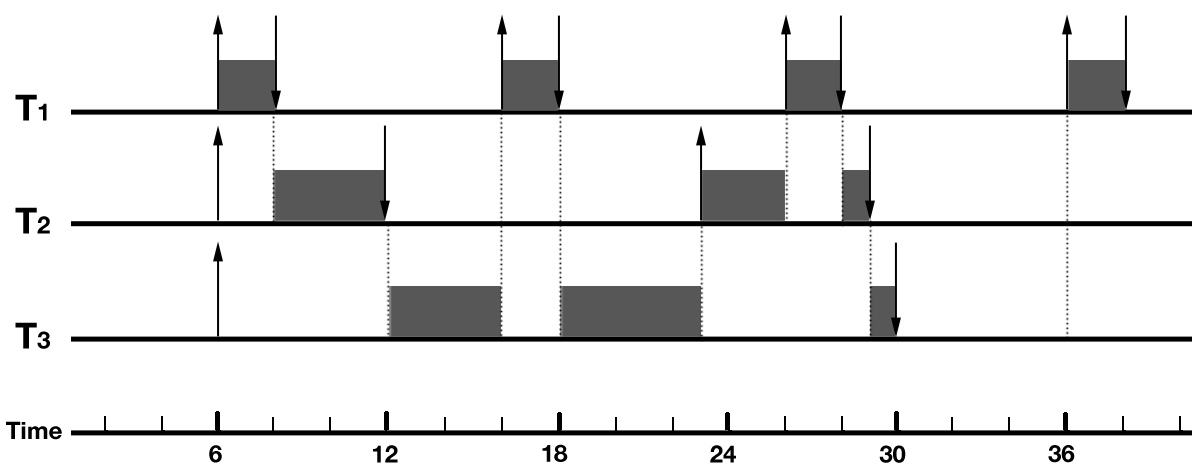
\includegraphics[scale=0.4]{1_2}
	\caption{Critical instant schedule, corresponding to assignment 1.2. All tasks can be scheduled.}
	\label{1_2}
	\end{figure}
	
	\item \emph{Assume that we want to increase the computation time for task $\tau_1$ to be $C_1 = 4$. Will all tasks complete before their deadlines? Draw a critical instant schedule for the given tasks. What is the system utilization bound?}
	
	\answer $U_1$ is now 0.4, giving $U = 0.9523$, which is larger than $U_{threshold} = 0.7797$, which means that it is not guaranteed to be schedulable according to the formula.

	\begin{figure}
	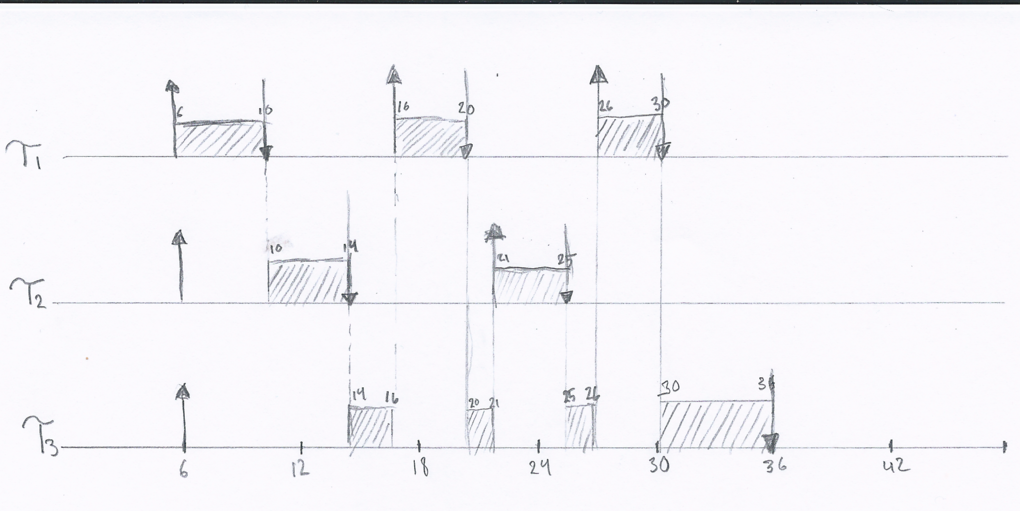
\includegraphics[scale=0.4]{1_3_low}
	\caption{Critical instant schedule, corresponding to assignment 1.3}
	\label{1_3}
	\end{figure}

	At time 36, all tasks have finished, thus this is schedulable according to our assumption about critical instants, as shown in figure \ref{1_3}.
	
	\item \emph{Assume that we want to increase the computation time for task $\tau_1$ to be $C_1 = 5$. Will all tasks complete before their deadlines? Draw a critical instant schedule for the given tasks. What is the system utilization bound?}
	
	\answer $U_1$ is now $0.5$, giving us $U = 1.0523$, again not guaranteed to be schedulable.
	
	\begin{figure}
	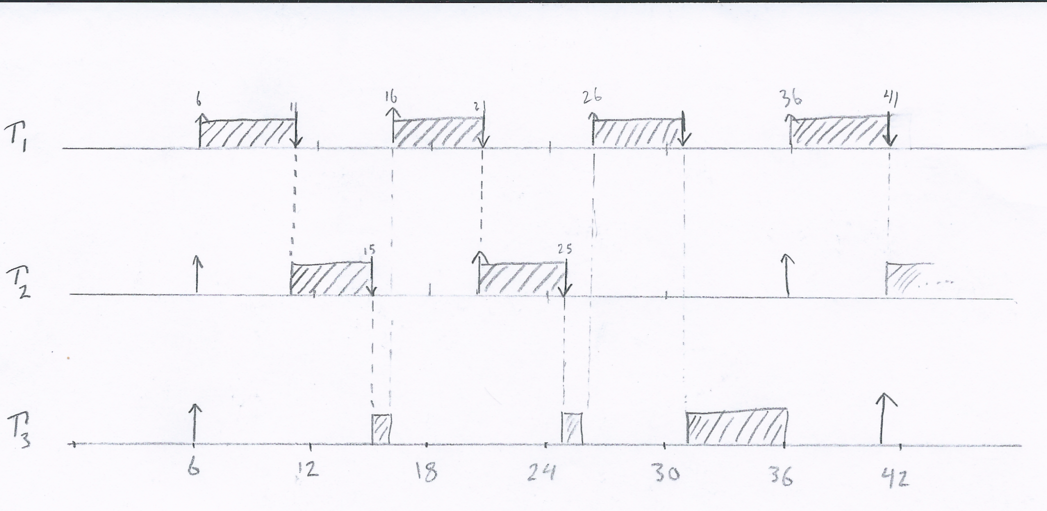
\includegraphics[scale=0.4]{1_4_low}
	\caption{Critical instant schedule, corresponding to assignment 1.4. $\tau_3$ misses its deadline at 41.}
	\label{1_4}
	\end{figure}
	
	At time 41, $\tau_3$ should have finished, but has only executed for $6 ms$ of the total of $10 ms$. Therefore $C_1 = 5$ is not schedulable, see figure \ref{1_4}.
	
	\item \emph{Assume that we instead of modifying $\tau_1$ (set $C_1 = 2$), want to increase the computation time for task $\tau_3$ to be $C_3 = 17$. Will all tasks complete before their deadlines? Draw a critical instant schedule for the given tasks. What is the system utilization bound?}
	
	\answer $U_3 = \frac{17}{35} = 0.4857$, giving $U = 0.9523$.
	
	\begin{figure}
	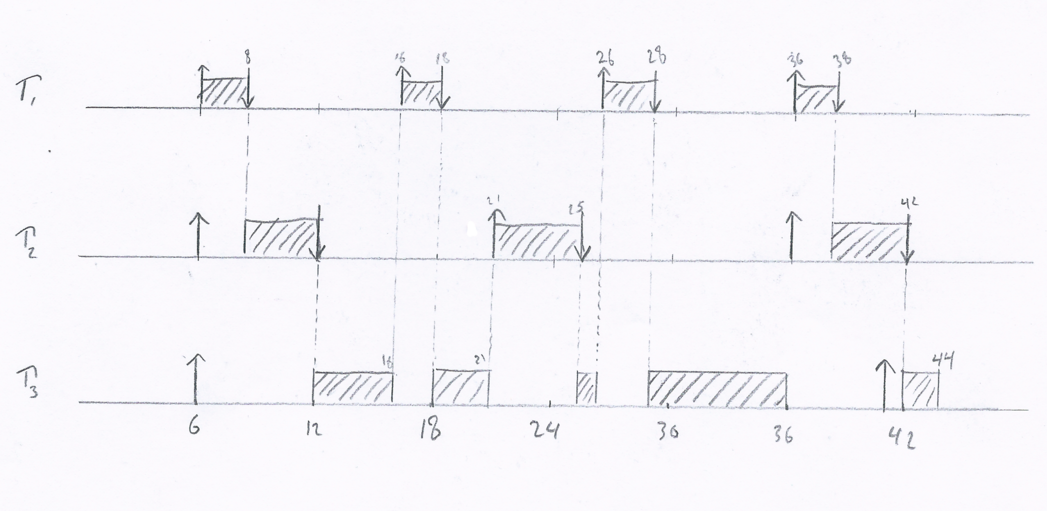
\includegraphics[scale=0.4]{1_5_low}
	\caption{Critical instant schedule, corresponding to assignment 1.5. $\tau_3$ again misses its deadline at 41.}
	\label{1_5}
	\end{figure}
	
	$\tau_3$ had a deadline at 41, but has only executed $15 ms$ at that time, see figure \ref{1_5}. It did therefore not meet its deadline, even though the utilization was exactly the same as in 1.3, which turned out to be schedulable.
	
	\item \emph{What conclusion can you draw from all this for the schedulability formula?}
	
	\answer Formula 2 is a sufficient formula, not a necessary one. If the utilization is higher than $n(2^{1/n}-1)$, it might still be possible to schedule, but when it is lower, it is guaranteed.
	
	The utilization must always be lower than 1 to be schedulable, as a higher number means we need more processing time than we have available.
	
	\item \emph{Insert the task set given in FpsCalc and calculate the response time of each task. What is the worst-case response time for each task using FpsCalc? Verify that the times correspond to the times you extracted using a critical instant schedule. In the worst case schenario, how many instances of $\tau_1$ and $\tau_2$ respectively can appear during one execution of $\tau_3$? How does this value relate to the $\ceil{\frac{R_i}{T_j}}$ expression? How long time of the worst case response time of $\tau_3$ is spent waiting for instances of $\tau_1$ and $\tau_2$ respectively?}
	
	\answer According to FpsCalc, $R_1 = 2$, $R_2 = 6$ and $R_3 = 24$ which is what we can see in the critical execution diagram in figure \ref{1_2}.
	
	During one execution of $\tau_3$, three executions of $\tau_1$ and two executions of $\tau_2$ can occur. These values are equal to the values $\ceil{\frac{R_i}{T_j}}$ for $j = 1, 2 \quad j \in \{1,2\}$. In the case of $\tau_3$:
	
	$\ceil{\frac{R_3}{T_1}} = \ceil{\frac{24}{10}} = 3$ and $\ceil{\frac{R_3}{T_2}} = \ceil{\frac{24}{15}} = 2$.
	
	The time we wait for other executions is the difference between the response time and the worst-case execution time. In this case:
	
	$R_3 - C_3 = 24 - 10 = 14$
	
	The code used to calculate the above values follows:
	
\begin{lstlisting}
  system testing {
    declarations {		
      indexed Period, Deadline, CompTime, RespTime;
      priority Priovar;	
      tasks A, B, C;
    }
    initialise {
      Period[A] = 10;
      Period[B] = 15;
      Period[C] = 35;
      
      Deadline[A] = 10;
      Deadline[B] = 15;
      Deadline[C] = 35;
      
      Priovar[A] = 1;
      Priovar[B] = 2;
      Priovar[C] = 3;
      
      CompTime[A] = 2;
      CompTime[B] = 4;
      CompTime[C] = 10;
    }
    formulas {
      RespTime[i] = CompTime[i] +
      sigma(hp, ceiling(RespTime[i] / Period[j]) * CompTime[j]);
    }
  }				   
\end{lstlisting}

When running this in FpsCalc, we get the following output:

\begin{lstlisting}[language=bash]
This is fpscalc version 2.02 1997

System 'testing'
-------------------

RespTime[A] = 2.000000
RespTime[B] = 6.000000
RespTime[C] = 24.000000
\end{lstlisting}

To save space, the FpsCalc printouts will be omitted in future exercises.

\end{enumerate}

\section{Assignment 2: Deadline Monotonic and Rate Monotonic Analysis}

\begin{enumerate}
	\item \emph{Given the task set, what is the priority ordering for the tasks using the DM priority ordering? What is the priority ordering using RM priority ordering? Use FpsCalc to calculate the response time for the tasks in both orderings. Will all tasks complete before their deadlines?}
	
	\answer The priority ordering for the tasks are:
	
	DM: $\tau_1$, $\tau_2$, $\tau_3$, $\tau_4$.
	RM: $\tau_2$, $\tau_3$, $\tau_1$, $\tau_4$.
	
	All priority listings in this report are written from highest (left) to lowest (right). With DM scheduling, it is schedulable with response times $R_1 = 2$, $R_2 = 5$, $R_3 = 13$ and $R_4 = 54$. With RM scheduling, the response times are $R_1 = 13$, $R_2 = 3$, $R_3 = 11$, $R_4 = 54$, which means that $\tau_1$ did not meet its deadline at $6ms$, when run with RM.
	
	The Deadline-monotonic values are calculated using the following FpsCalc definition file:

        \begin{lstlisting}
          system testing {
            declarations {		
              indexed Period, Deadline, CompTime, RespTime;
              priority Priovar;	
              
              tasks A, B, C, D;
            }
            
            initialise {
              Period[A] = 20;
              Period[B] = 7;
              Period[C] = 14;
              Period[D] = 100;
              
              Deadline[A] = 6;
              Deadline[B] = 7;
              Deadline[C] = 13;
              Deadline[D] = 60;
              
              Priovar[A] = 1;
              Priovar[B] = 2;
              Priovar[C] = 3;
              Priovar[D] = 4;
              
              CompTime[A] = 2;
              CompTime[B] = 3;
              CompTime[C] = 5;
              CompTime[D] = 4;
              
            }
            
            formulas {
              RespTime[i] = CompTime[i] +
              sigma(hp, ceiling(RespTime[i] / Period[j]) * CompTime[j]);
            }
          }
        \end{lstlisting}
        
        The same definition file is used to calculate the Rate-monotonic, but with the priorities changed as follows:
        
        \begin{lstlisting}
          Priovar[A] = 3;
		  Priovar[B] = 1;
		  Priovar[C] = 2;
		  Priovar[D] = 4;
        \end{lstlisting}

	\item \emph{Sometimes it is preferable to not use strict RM or DM priority assignment when giving priorities to tasks. This can for example happen when we want to give a task with low deadline demands a better service rate or when the system is part of a larger distributed system. Find two different priority assignments of the tasks which is neither RM or DM and where deadlines are missed and met respectively.}
	
	\answer One order is $\tau_2$, $\tau_1$, $\tau_3$, $\tau_4$ which gives us the response times 
	
	$R_1 = 5 (< 6)$, $R_2 = 3 (< 7)$, $R_3 = 13 (= 13)$ and $R_4 = 54 (< 60)$. 
	
	This means that all tasks meet their deadlines. The FpsCalc definition for this result is:

        \begin{lstlisting}
          system testing {
            declarations {		
              indexed Period, Deadline, CompTime, RespTime;
              priority Priovar;	
              
              tasks A, B, C, D;
            }
            
            initialise {
              Period[A] = 20;
              Period[B] = 7;
              Period[C] = 14;
              Period[D] = 100;
              
              Deadline[A] = 6;
              Deadline[B] = 7;
              Deadline[C] = 13;
              Deadline[D] = 60;
              
              Priovar[A] = 2;
              Priovar[B] = 1;
              Priovar[C] = 3;
              Priovar[D] = 4;
              
              CompTime[A] = 2;
              CompTime[B] = 3;
              CompTime[C] = 5;
              CompTime[D] = 4;
            }
            
            formulas {
              RespTime[i] = CompTime[i] +
              sigma(hp, ceiling(RespTime[i] / Period[j]) * CompTime[j]);
            }
          }
        \end{lstlisting}

	
	Another order is $\tau_1$, $\tau_3$, $\tau_2$, $\tau_4$, which will lead to $\tau_2$ not meeting its deadline. The response times are
	
	$R_1 = 2 (< 6)$, $R_2 = 10 (> 7)$, $R_3 = 7 (< 13)$ and $R_4 = 54 (< 60)$.
	The FpsCalc definition file used to calculate this is the same as the previous, except that the priorities have been exchanged as follows:

        \begin{lstlisting}
          Priovar[A] = 1;
          Priovar[B] = 3;
          Priovar[C] = 2;
          Priovar[D] = 4;
        \end{lstlisting}
	
	\item \emph{Assume that we want to implement the tasks on a RT-kernel that only supports 3 priority levels and where tasks with the same priority will be handled in FIFO order by the scheduler. Assume that task $\tau_2$ and $\tau_3$ are set to have the same priority and that we use a DM priority assignment.}
	
	\emph{Define how the response time formula will be changed when we allow several tasks to have the same priority. Make sure that it is shown in your formula that a task, du to the FIFO order, might have to wait for one instance, but can't be preempted, of an equal priority task. What will the corresponding FpsCalc formula look like?}
	
	\emph{What will now the worst case response time for each task be? Will all tasks meet their deadlines? Will the worst case response time for task $\tau_1$ or $\tau_4$ be affected? Conclusions?}
	
	\answer The formula will now be (assuming that the current task is included in $ep(i)$):
	
	\begin{equation*}
		R_i = \sum_{j \in hp(i)}{\ceil{\frac{R_i}{T_j}}C_j} + \sum_{j \in ep(i)}{C_j}
	\end{equation*}
	
	Since $\tau_i$ is a task with the same priority as itself, the constant $C_i$ is removed. The second sum shows that a task with equal priority will be run at most once before $\tau_i$, thus the ceiling operator is not needed.
	
	For the example, the worst-case response times are
	
	$R_1 = 2 (< 6)$, $R_2 = 10 (> 7)$, $R_3 = 10 (< 13)$ and $R_4 = 54 (< 60)$.
	
	We see that the response times of $\tau_1$ and $\tau_4$ are unaffected. $\tau_3$ will always meet is deadline, but $\tau_2$ will not, if $\tau_3$ reaches the FIFO-queue before $\tau_2$ does.
	
	In FpsCalc, the formula is:
	
	\begin{lstlisting}
          RespTime[i] =
          sigma(hp, ceiling(RespTime[i] / Period[j]) * CompTime[j])
          + sigma(ep, CompTime[j])
	\end{lstlisting}

        The rest of the FpsCalc definition file is the same as for the previous excercise, with the change that $\tau_2$ and $\tau_3$ now have the same priorities.
	
	We can conclude that fixed priority-level machines might affect performance. Also, the worst-case response time of all tasks with the same priority will be the same.
	
\end{enumerate}

\section{Assignment 3: Context Switch Time}

\begin{enumerate}
	\item \emph{Extend the response time formula with the time to do context switches between tasks. Use the $C_{save}$ and $C_{load}$ parameters in your formula. This means that each task's computation time must first be extended to include the extra context switch time needed to first load and finally save the task. After that you must extend your response time formula to (pessimistically) include the extra context switch time each preemption from a higher priority task will result in. A task must be able to save its context before its deadline.}
	
	\answer The formula for taking context switch times into consideration is:
	
	\begin{equation*}
	R_i = C_i + C_{save} + C_{load} + \sum_{j \in hp(i)}{\ceil{\frac{R_i}{T_j}} (C_j + 2(C_{save} + C_{load}))}
	\end{equation*}
	
	This formula expressed in the FpsCalc definition file is:
	
	\begin{lstlisting}
          WCRespTimeCS[i] =
          CompTime[i] + CSload + CSsave 
          + sigma(hp, ceiling(WCRespTimeCS[i] / Period[j]) * (CompTime[j]
          + 2 * (CSload + CSsave)));
	\end{lstlisting}
	
	\item \emph{To illustrate the time needed for context switches, draw a scheme where a task $\tau_i$ arrives and starts executing for the first time, executes for a while, gets preempted by a higher priority task $\tau_j$, which also executes for a while. When $\tau_j$ has completed its execution $\tau_i$ will continue its execution until it is done. Make sure that you clearly show that there is a difference from when a task arrives until it starts to execute. Make also sure that the times for loading contexts, saving contexts, and executing normally are distinguishable. Finally, make sure that your extended schedulability formula in 1 actually captures all time used for context switching.}
	
	\answer 
	
	
	\begin{figure}
	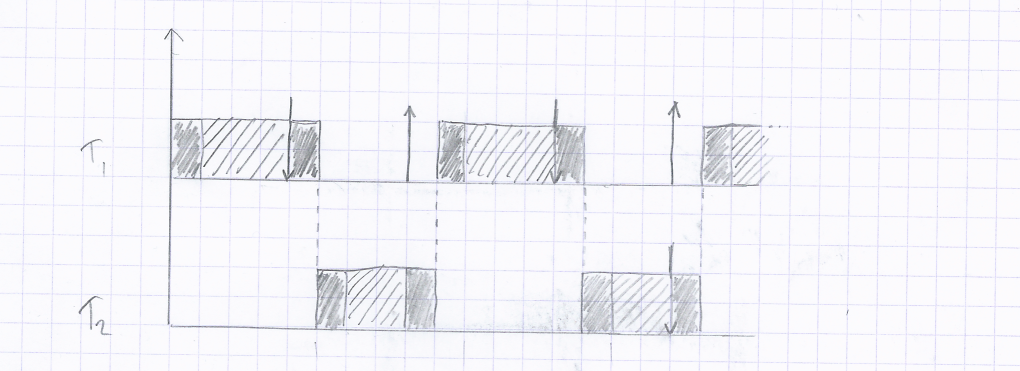
\includegraphics[scale=0.4]{3_2_low}
	\caption{Critical instant schedule, corresponding to assignment 3.2.}
	\label{3_2}
	\end{figure}
	
	We use the following definition file to calculate the worst case response times for $\tau_i$ and $\tau_j$:
	
	\begin{lstlisting}
	scalar CSload, CSsave;

	system testing {
		declarations {
			indexed Period, Deadline, CompTime, WCRespTimeCS;
			priority Priovar;
			  
			tasks A, B;
		}

		initialise {
			Period[A] = 9;
			Period[B] = 32;

			Deadline[A] = 9;
			Deadline[B] = 32;

			Priovar[A] = 1;
			Priovar[B] = 2;

			CompTime[A] = 3;
			CompTime[B] = 4;

			CSload = 1;
			CSsave = 1;
		}

		formulas {
			WCRespTimeCS[i] = CompTime[i] + CSload + CSsave +
				sigma(hp, ceiling(WCRespTimeCS[i] / Period[j]) * (CompTime[j] + 
				2 *(CSload + CSsave)));
		}
	}
	\end{lstlisting}
	
	The values calculated by FpsCalc using our formula from 3.1 gives the answers below:
	
	\begin{lstlisting}[language=bash]
	This is fpscalc version 2.02 1997

	System 'testing'
	-------------------
	WCRespTimeCS[A] = 5.000000
	WCRespTimeCS[B] = 27.000000
	\end{lstlisting}

	The results do not perfectly match the values from the image, since the schedulability formula is pessimistic, and will add an extra context switch when the two tasks are initialized at time zero. This allows $\tau_1$ to run once more before $\tau_2$ has finished in comparison to picture \ref{3_2}
	
	\item \emph{Assume that $C_{save} = C_{load} = 0.1 ms$ for the system. What are the worst case response times for the tasks (using DM priority order) when including the time for doing context switches? Are all deadlines met?}
	
	\answer The deadlines are not all met. The results were:
	
	$R_1 = 2.2 (<6)$, $R_2 = 5.6 (<7)$, $R_3 = 17.8 (>13)$ and $R_4 = 518 (>60)$.
	
	$R_3$ and $R_4$ show that two tasks may miss their deadlines.

        The FpsCalc definition file used for these calculations is:

        \begin{lstlisting}
          scalar CSload, CSsave;
          
          system testing {
            declarations {		
              indexed Period, Deadline, CompTime, WCRespTimeCS;
              priority Priovar;	
              
              tasks A, B, C, D;
            }
            
            initialise {
              Period[A] = 20;
              Period[B] = 7;
              Period[C] = 14;
              Period[D] = 100;
              
              Deadline[A] = 6;
              Deadline[B] = 7;
              Deadline[C] = 13;
              Deadline[D] = 60;
              
              Priovar[A] = 1;
              Priovar[B] = 2;
              Priovar[C] = 3;
              Priovar[D] = 4;
              
              CompTime[A] = 2;
              CompTime[B] = 3;
              CompTime[C] = 5;
              CompTime[D] = 4;
              
              CSload = 0.1;
              CSsave = 0.1;
            }
            
            formulas {
              WCRespTimeCS[i] = CompTime[i] + CSload + CSsave + 
              sigma(hp, ceiling(WCRespTimeCS[i] / Period[j]) * (CompTime[j] + 2 *(CSload + CSsave))); 
            }
          }
        \end{lstlisting}
	
\end{enumerate}

\section{Assignment 4: Blocking}

\begin{enumerate}
	\item \emph{Give priorities to the tasks according to the DM priority assignment. Will all tasks always meet their deadlines?}
	
	\answer The priorities are $\tau_1$, $\tau_2$, $\tau_3$, $\tau_4$. They are schedulable, with $R_1 = 2 (<5)$, $R_2 = 5 (<12)$, $R_3 = 17 (< 40)$ and $R_4 = 26 (<50)$.

        The response times have been calculated using the following FpsCalc definition file:

        \begin{lstlisting}
          system testing {
            declarations {		
              indexed Period, Deadline, CompTime, RespTime;
              priority Priovar;	
              
              tasks A, B, C, D;
            }
            
            initialise {
              Period[A] = 10;
              Period[B] = 20;
              Period[C] = 40;
              Period[D] = 100;
              
              Deadline[A] = 5;
              Deadline[B] = 12;
              Deadline[C] = 40;
              Deadline[D] = 50;
              
              Priovar[A] = 1;
              Priovar[B] = 2;
              Priovar[C] = 3;
              Priovar[D] = 4;
              
              CompTime[A] = 2;
              CompTime[B] = 3;
              CompTime[C] = 10;
              CompTime[D] = 4;
            }
            
            formulas {
              RespTime[i] = CompTime[i] +
              sigma(hp, ceiling(RespTime[i] / Period[j]) * CompTime[j]);
            }
          }
        \end{lstlisting}

	\item \emph{Assume that task $\tau_2$ and $\tau_4$ are sharing a semaphore $S_1$, and that $\tau_2$ and $\tau_4$ executes for at most $1 ms$ and $2 ms$ respectively in the critical section. Show, by doing a critical instant scheme that the deadline for task $\tau_2$ can be missed if semaphores and no mechanism for limiting priority inversion is used.}
	
	\answer In figure \ref{4_2} we see a critical instant schedule modelling this situation. The process $\tau_4$ locks the semaphore, and blocks $\tau_2$. Since $\tau_3$ has higher priority than $\tau_2$, both $\tau_4$ and $\tau_2$ are delayed, causing $\tau_2$ to miss its deadline at 12.

	\begin{figure}
	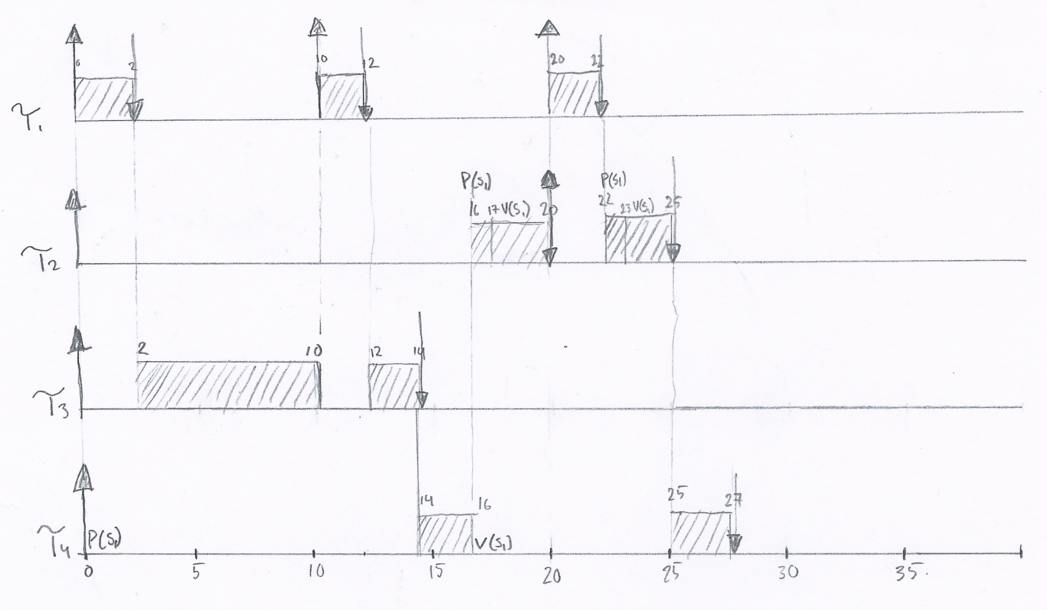
\includegraphics[scale=0.4]{4_2_low}
	\caption{Critical instant schedule, corresponding to assignment 4.2. $\tau_2$ misses its deadline at 12.}
	\label{4_2}
	\end{figure}

	\item \emph{Assume that task $\tau_2$ not only is sharing a semaphore $S_1$ with $\tau_4$ but also is sharing a semaphore $S_2$ with task $\tau_3$. Also assume that the times the task $\tau_2$ is accessing the semaphores $S_1$ and $S_2$ do not overlap. Show, by doing a critical instant scheme that deadline for task $\tau_2$ can be missed even though the priority inheritance protocol is used.}
	
	\answer In figure \ref{4_3} we see that $\tau_2$ still can miss its deadline, completing at 14 when the deadline is set at 12. This is because it is blocked not only by $\tau_4$, but also by $\tau_3$ for the times they use the semaphores.

	\begin{figure}
	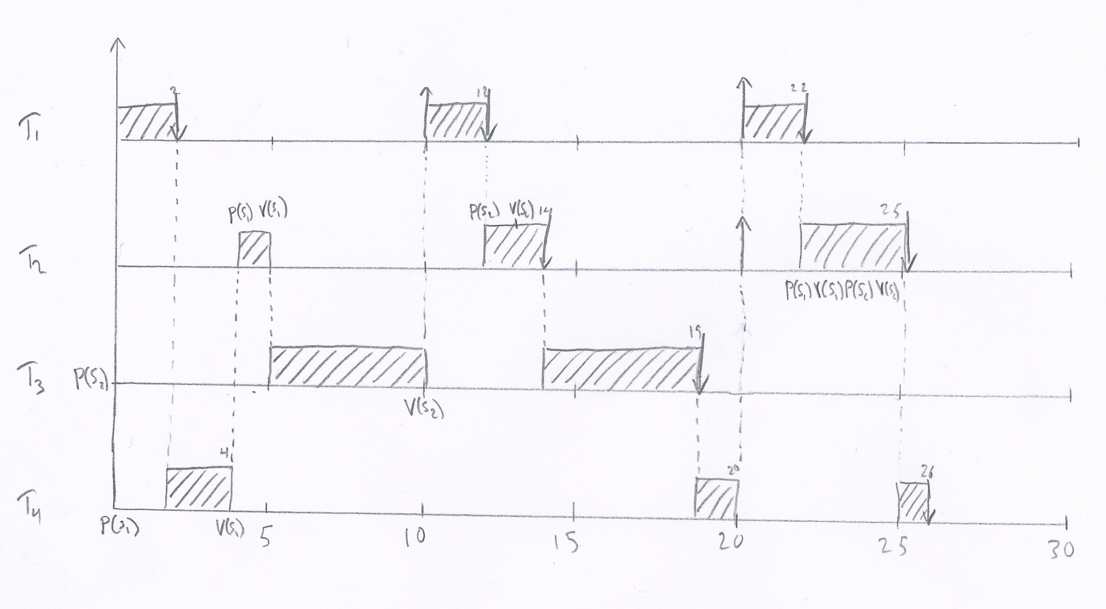
\includegraphics[scale=0.4]{4_3_low}
	\caption{Critical instant schedule, corresponding to assignment 4.3. $\tau_2$ again misses its deadline at 12.}
	\label{4_3}
	\end{figure}

	\item \emph{What are the blocking times for the tasks using the priority inheritance protocol? Make sure that the amount of blocking corresponds to your drawn schedule.}
	
	\answer The $B_1 = 0$, as it has the highest priority and uses no semaphores. Likewise, $B_4 = 0$, as it has the lowest priority and will only run once the other tasks are not running. Then $B_3 = 2$ which is the time it might be blocked by $\tau_4$, and $B_2 = 7$, which is the time it might be blocked by $\tau_4$ and $\tau_3$.
	
	\item \emph{What are the priority ceilings for the semaphores $S_1$ and $S_2$? What are the blocking times for the tasks using the immediate inheritance protocol? Explain why task $\tau_3$ can experience blocking even though it does not share any semaphore with $\tau_4$. Will all tasks complete before their deadlines?}
	
	\answer The priority ceiling is 2, both for $S_1$ and $S_2$, as $\tau_2$ uses both semaphores and has the highest priority among those using the semaphores. As before, $B_1$ and $B_4$ are zero. $B_2 = 5$, because it can be blocked either by $\tau_3$ or $\tau_4$ and we chose the more pessimistic value as the blocking time. Lastly, $B_3 = 2$, which is the time it can be blocked by $\tau_4$. Even though $\tau_3$ has a higher priority than $\tau_4$ and doesn't share a semaphore with $\tau_4$, if $\tau_4$ blocks $\tau_2$ it will in effect also block $\tau_3$.
	
	\begin{figure}
	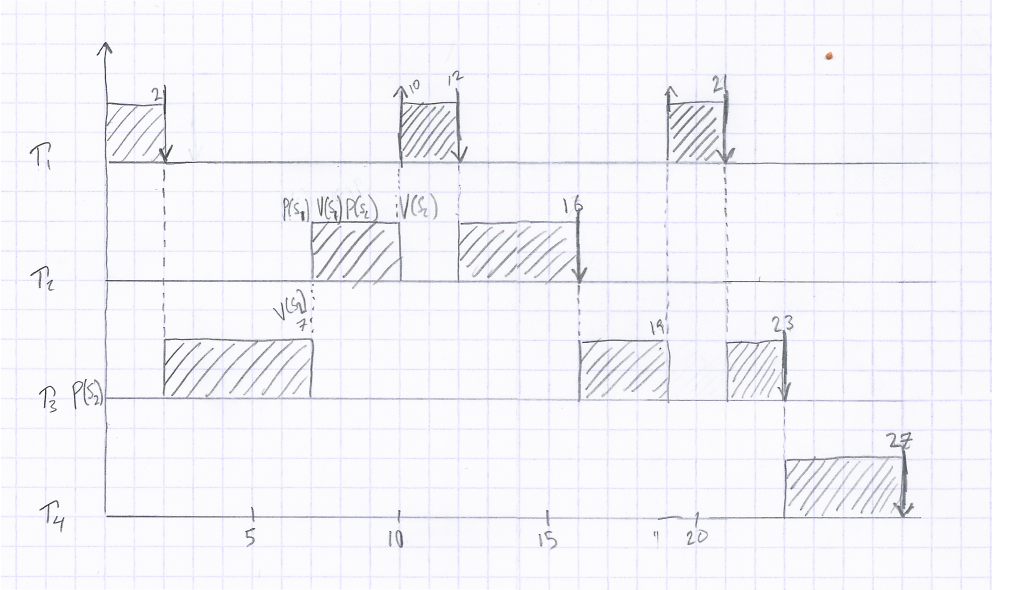
\includegraphics[scale=0.4]{3_5_low}
	\caption{Critical instant schedule, corresponding to assignment 4.5.}
	\label{4_5}
	\end{figure}

	All tasks will complete before the deadline using this protocol: $R_1 = 2 (<5)$, $R_2 = 10 (<12)$, $R_3 = 17 (<40)$ and $R_4 = 26 (<50)$ regardless which of the tasks blocks $\tau_2$. See figure \ref{4_5}.
\end{enumerate}

\section{Assignment 5: Jitter}

\begin{enumerate}
	\item \emph{A source of jitter is varying execution and response times for tasks (or messages) that start other tasks. To illustrate this assume a system with two tasks $\tau_1$ and $\tau_2$. Let task $\tau_1$ have a period $T_1 = 10$ and a fixed (non-varying) execution time $C_1 = 3$. Let task $\tau_2$ always arrive 2 time units after $\tau_1$ arrives, but it waits for $\tau_1$ finishing before it gets released. Assume task $\tau_1$ always ends its execution by releasing task $\tau_2$. Let $\tau_2$ have a worst case execution time of $C_2 = 2$.}
	
	\emph{Draw a schedule that shows two instances of $\tau_1$ and $\tau_2$ respectively. What is the period $T_2$ of task $\tau_2$?}
	
	\answer
	
	\begin{figure}
	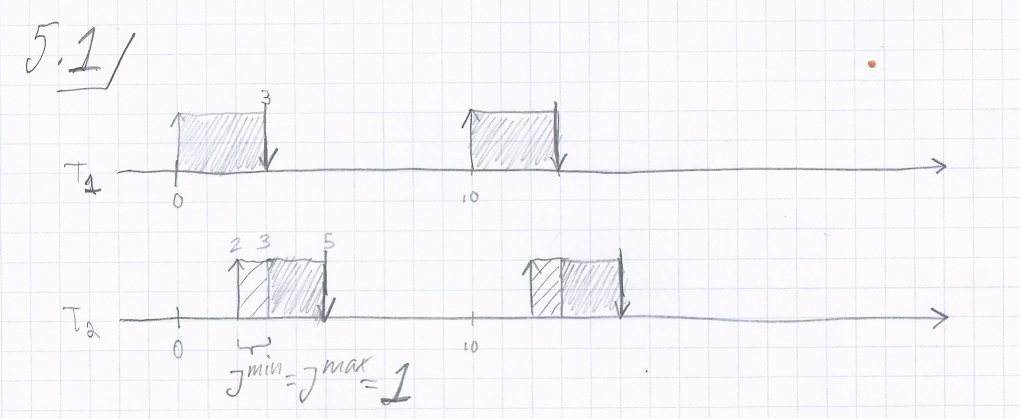
\includegraphics[scale=0.4]{5_1_low}
	\caption{Critical instant schedule depicting the case where there is no jitter, corresponding to assignment 5.1.}
	\label{5_1}
	\end{figure}
	
	Figure \ref{5_1} shows $\tau_1$ and $\tau_2$ running. Since $T_1 = 10$ and $\tau_2$ arrives two time units after $\tau_1$, $T_2 = 10$ also.
	
	\item \emph{To illustrate that varying execution time of $\tau_1$ might cause jitter of $\tau_2$ assume that $\tau_1$'s execution time no longer is fixed but varies between $C_1^{min} = 3$ and $C_1^{max} = 5$. Task $\tau_1$ still starts task $\tau_2$ at the end of its execution.}
	
	\emph{Draw a schedule with two instances of $\tau_1$ that shows that the varying execution time of $\tau_1$ might give raise to jitter of $\tau_2$. What is the jitter that task $\tau_2$ can experience?}
		
	\answer Since the execution time of $\tau_1$ can vary with 2 time units, $J_2 = 2$. An execution showing the two extreme cases can be seen in figure \ref{5_2}.
	
	\begin{figure}
	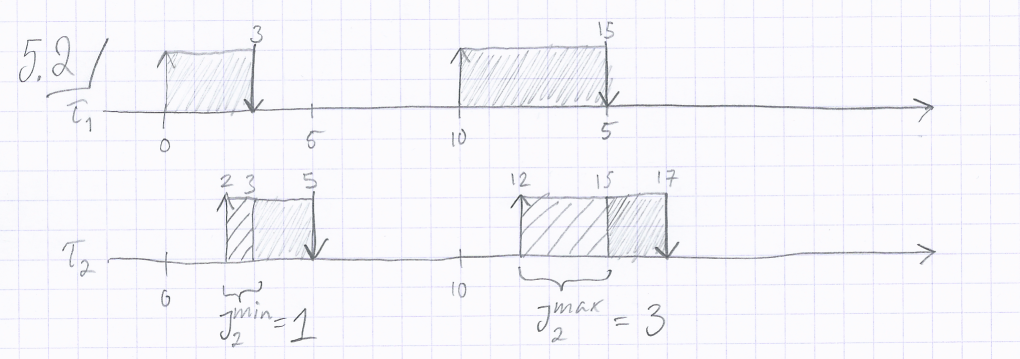
\includegraphics[scale=0.4]{5_2_low}
	\caption{Critical instant schedule depicting the case where $\tau_1$ has varying execution time, corresponding to assignment 5.2.}
	\label{5_2}
	\end{figure}
	
	\item \emph{To illustrate that interference of high priority tasks might give raise to further jitter of low priority tasks we add a task $\tau_0$ to the system. Let task $\tau_0$ have higher priority than both $\tau_1$ and $\tau_2$, a period $T_0 = 20$ and a worst case execution time $C_0 = 2$.}
	
	\emph{Draw a schedule that shows that varying response time of $\tau_1$ due to interference of $\tau_0$ will give raise to further jitter of $\tau_2$. Task $\tau_1$'s execution time still varies between $C_1^{min}$ and $C_1^{max}$. What is the jitter that $\tau_2$ can experience due to varying response and execution time of $\tau_1$?}
	

	\answer Compared to the previous question, $\tau_1$ has varying execution times. Due to the jitter, $\tau_0$ may be released and run before $\tau_2$ as it has higher priority. Thus $J_2^{min} = 1$ and $J_2^{max} = 5$ giving $J_2 = 4$. This situation is illustrated in figure \ref{5_3}.
	
	\begin{figure}
	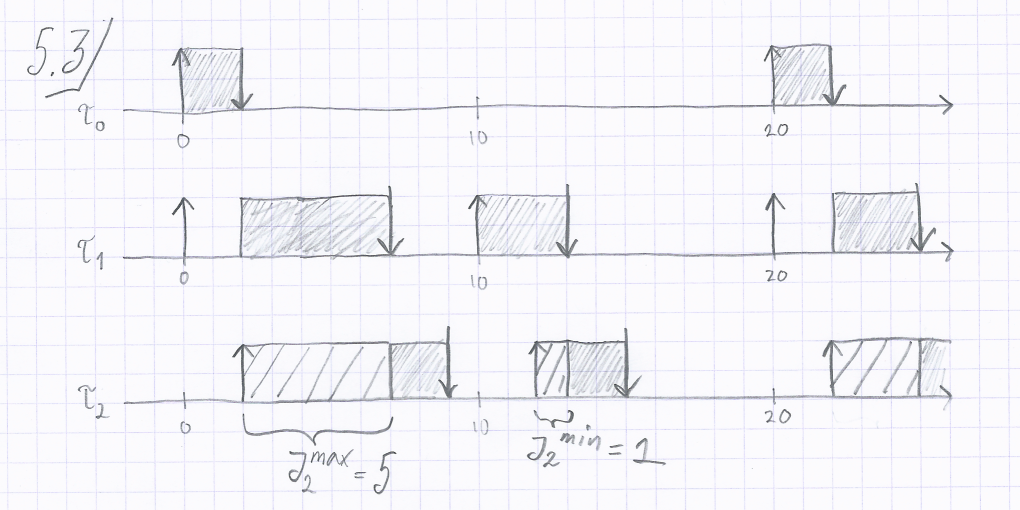
\includegraphics[scale=0.4]{5_3_low}
	\caption{Critical instant schedule depicting the case where $\tau_0$ may block $\tau_2$due to jitter in $\tau_1$, corresponding to assignment 5.3.}
	\label{5_3}
	\end{figure}	
	
	\item \emph{For the given tasks $\tau_A$ and $\tau_B$ with DM priority ordering, what is the worst case response time for respective task assuming that we have no jitter. Will both tasks be able to finish before their deadlines?}
	
	\answer The worst case response time for the tasks is $R_A = 5$ and $R_B = 40$. Since the deadlines are $D_A = 10$ and $D_B = 50$ both tasks will finish before their deadlines in all cases. The value was calculated by the \texttt{RespTime} formula in the following FpsCalc definition file:

	\begin{lstlisting}
          system testing {
            declarations {		
              indexed Period, Deadline, CompTime, RespTime, WCRespTimeJitter, RCRTJitter, Jitter;
              priority Priovar;	
              
              tasks A, B;
            }
            
            initialise {      
              Period[A] = 20;
              Period[B] = 50;
              
              Deadline[A] = 10;
              Deadline[B] = 50;
              
              Priovar[A] = 1;
              Priovar[B] = 2;
              
              CompTime[A] = 5;
              CompTime[B] = 30;
              
              Jitter[A] = 5;
              Jitter[B] = 10;
            }
            
            formulas {
              
              ! No jitter
              RespTime[i] = CompTime[i] + sigma(hp, ceiling(RespTime[i] / Period[j]) * CompTime[j]);
              
              ! Jitter. w-formula.
              RCRTJitter[i] = CompTime[i] + 
			    sigma(hp, ceiling((RCRTJitter[i] + Jitter[j]) / Period[j]) * CompTime[j]);
              
              ! Jitter. R-formula.
              WCRespTimeJitter[i] = RCRTJitter[i] + Jitter[i];
            }
          }
	\end{lstlisting}

	\item \emph{What is the worst case response time for respective tasks assuming that they can experience jitter? Will both tasks be able to complete before their deadlines?}
	
	\answer From the FpsCalc code in the previous excercise, we also get the worst case execution time for the tasks when taking jitter into account. The values calculated by the \texttt{WCRespTimeJitter} formula gives us the response times $R_A = 10 ms$ and $R_B = 55 ms$. Since the deadlines for the tasks are $D_A = 10 ms$ and $D_B = 50$, $\tau_B$ will miss its deadline.

	\item \emph{Draw a task schedule for the tasks $\tau_A$ and $\tau_B$ which gives the same worst case response times as the formula. Indicate arrival, jitter, beginning of execution, execution, preemption, and completion for each task in your schedule.}
	
	ANSWER
\end{enumerate}

\end{document}
